\documentclass[12pt]{report}

\usepackage[utf8]{inputenc}
\usepackage[T1]{fontenc}
\usepackage[francais]{babel}
\usepackage{setspace}
\usepackage[top=2.5cm,bottom=2.5cm,right=3cm,left=3cm]{geometry}

\usepackage{hyperref}
\usepackage{color}

\usepackage{calc}
\usepackage{pseudocode}

\usepackage{graphicx}

\AddThinSpaceBeforeFootnotes

\FrenchFootnotes

\title{Annexes - Rapport de stage}
\author{Antonin Carette}
\date{Compilé le \today}

\begin{document}

\maketitle

\tableofcontents

\chapter*{Préparation}

\addcontentsline{toc}{chapter}{Préparation}

\begin{figure}[h]
\begin{center}
\rotatebox{90}{
	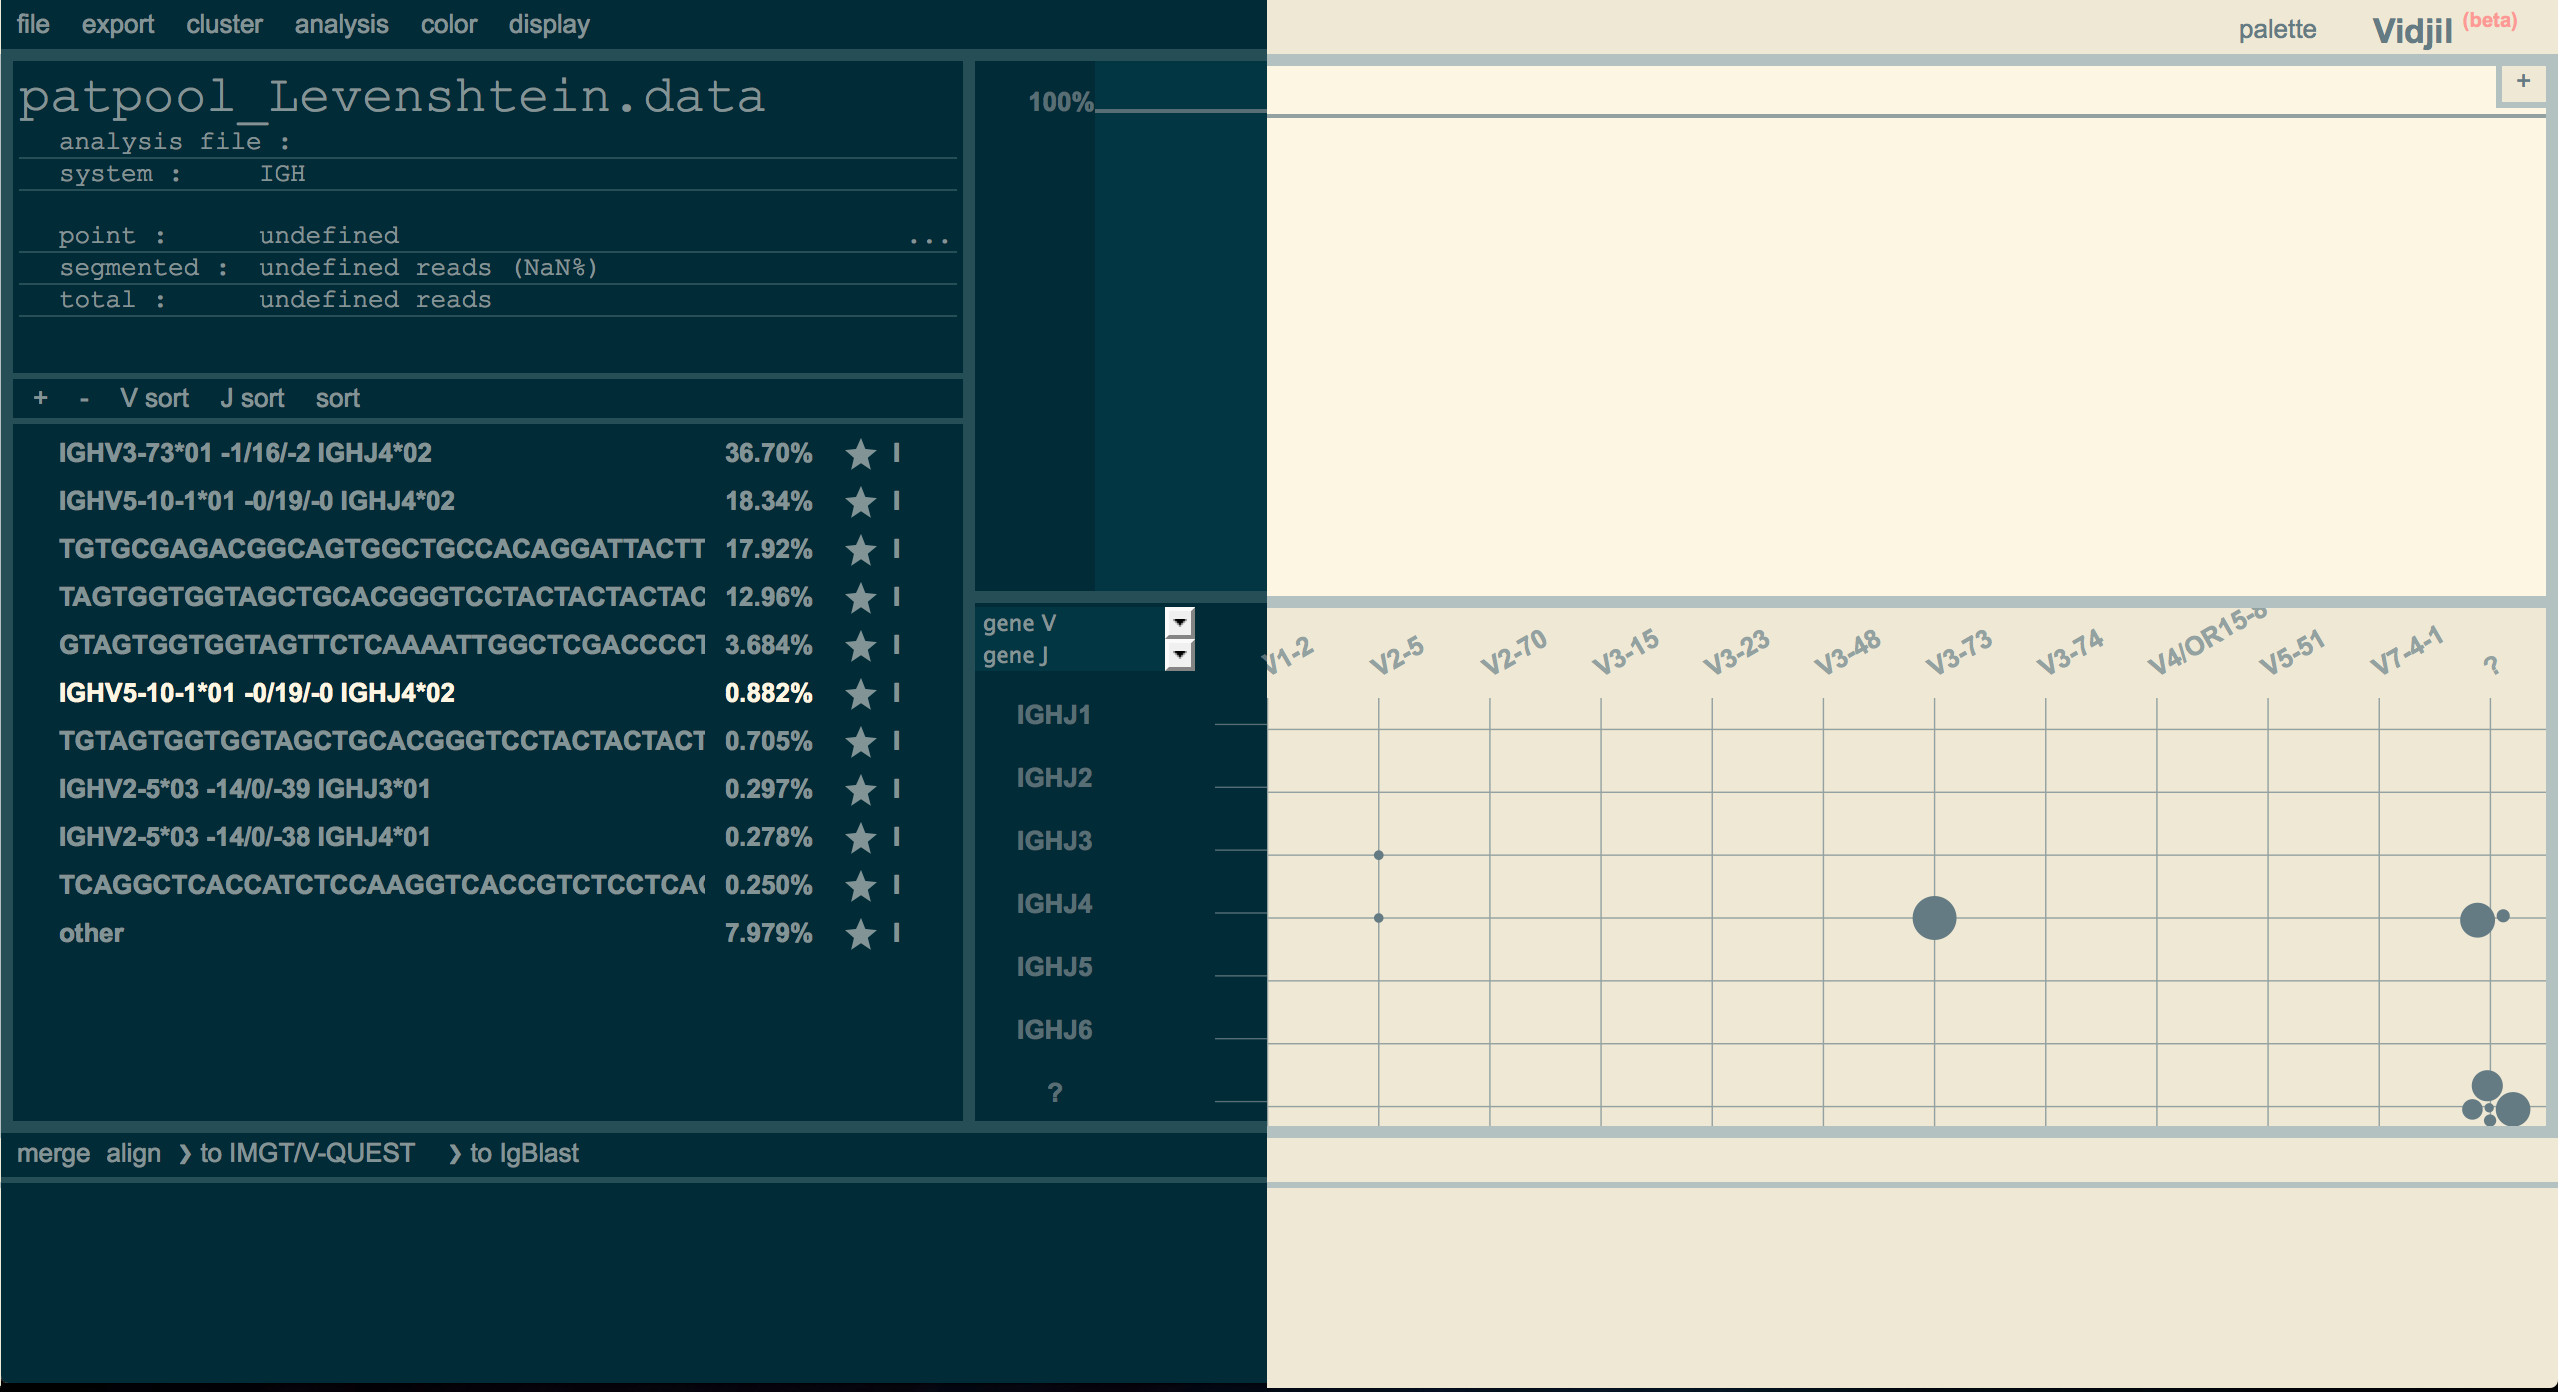
\includegraphics[scale=0.35]{img/Montage_Sans_Annotations.jpg}
}
\end{center}
\caption{Aperçu général de l'\textit{afficheur} - montage avec palette ``Dark'' et ``Light''}
\end{figure}

\chapter*{Le graphe de distances d'édition}

\addcontentsline{toc}{chapter}{Le graphe de distances d'édition}

\chapter*{DBSCAN}

\addcontentsline{toc}{chapter}{DBSCAN}

\begin{pseudocode}{DBSCAN}{D, eps, MinPts}
\COMMENT{Base de l'algorithme}\\
C $=$ 0\\
$Pour chaque point $P$ non visité des données $D\\
$marquer $P$ comme visité$\\
PtsVoisins$ = $\CALL{epsilonVoisinage}{P, eps}\\
\IF tailleDe(PtsVoisins) < MinPts
\THEN $marquer $P$ comme "bruit"$
\ELSE 
	\BEGIN
		C$++$\\
		\CALL{extensionCluster}{D, P, PtsVoisins, C, eps, MinPts}\\
	\END\\
\\

\COMMENT{Procédure permettant d'inclure un point dans un cluster - extension d'un cluster}\\
\PROCEDURE {extensionCluster}{D, P, PtsVoisins, C, eps, MinPts}
	$Ajouter $P$ au cluster C$\\
	\FOREACH P' \in PtsVoisins \DO
			\IF P'$ n'a pas été visité$
			\THEN 
				\BEGIN
					$Marquer $P'$ comme visité$\\
					PtsVoisins'$ = $ \CALL{epsilonVoisinage}{D, P', eps}\\
					\IF tailleDe(PtsVoisins') >= MinPts
					\THEN PtsVoisins$ = $PtsVoisins \cup PtsVoisins'\\
				\END\\
			\IF P'$ n'est membre d'aucun cluster$
			\THEN $Ajouter $P'$ au cluster $C
\ENDPROCEDURE

\COMMENT{Procedure retournant tous les points de $D$ qui sont à une distance inférieure à $eps$ de $P$}\\
\PROCEDURE{epsilonVoisinage}{D, P, eps}
	$Retourner tous les points de $D$ qui sont à une distance inférieure à $eps$ de $P
\ENDPROCEDURE
\end{pseudocode}

\begin{figure}[h]
\begin{center}
\rotatebox{90}{
	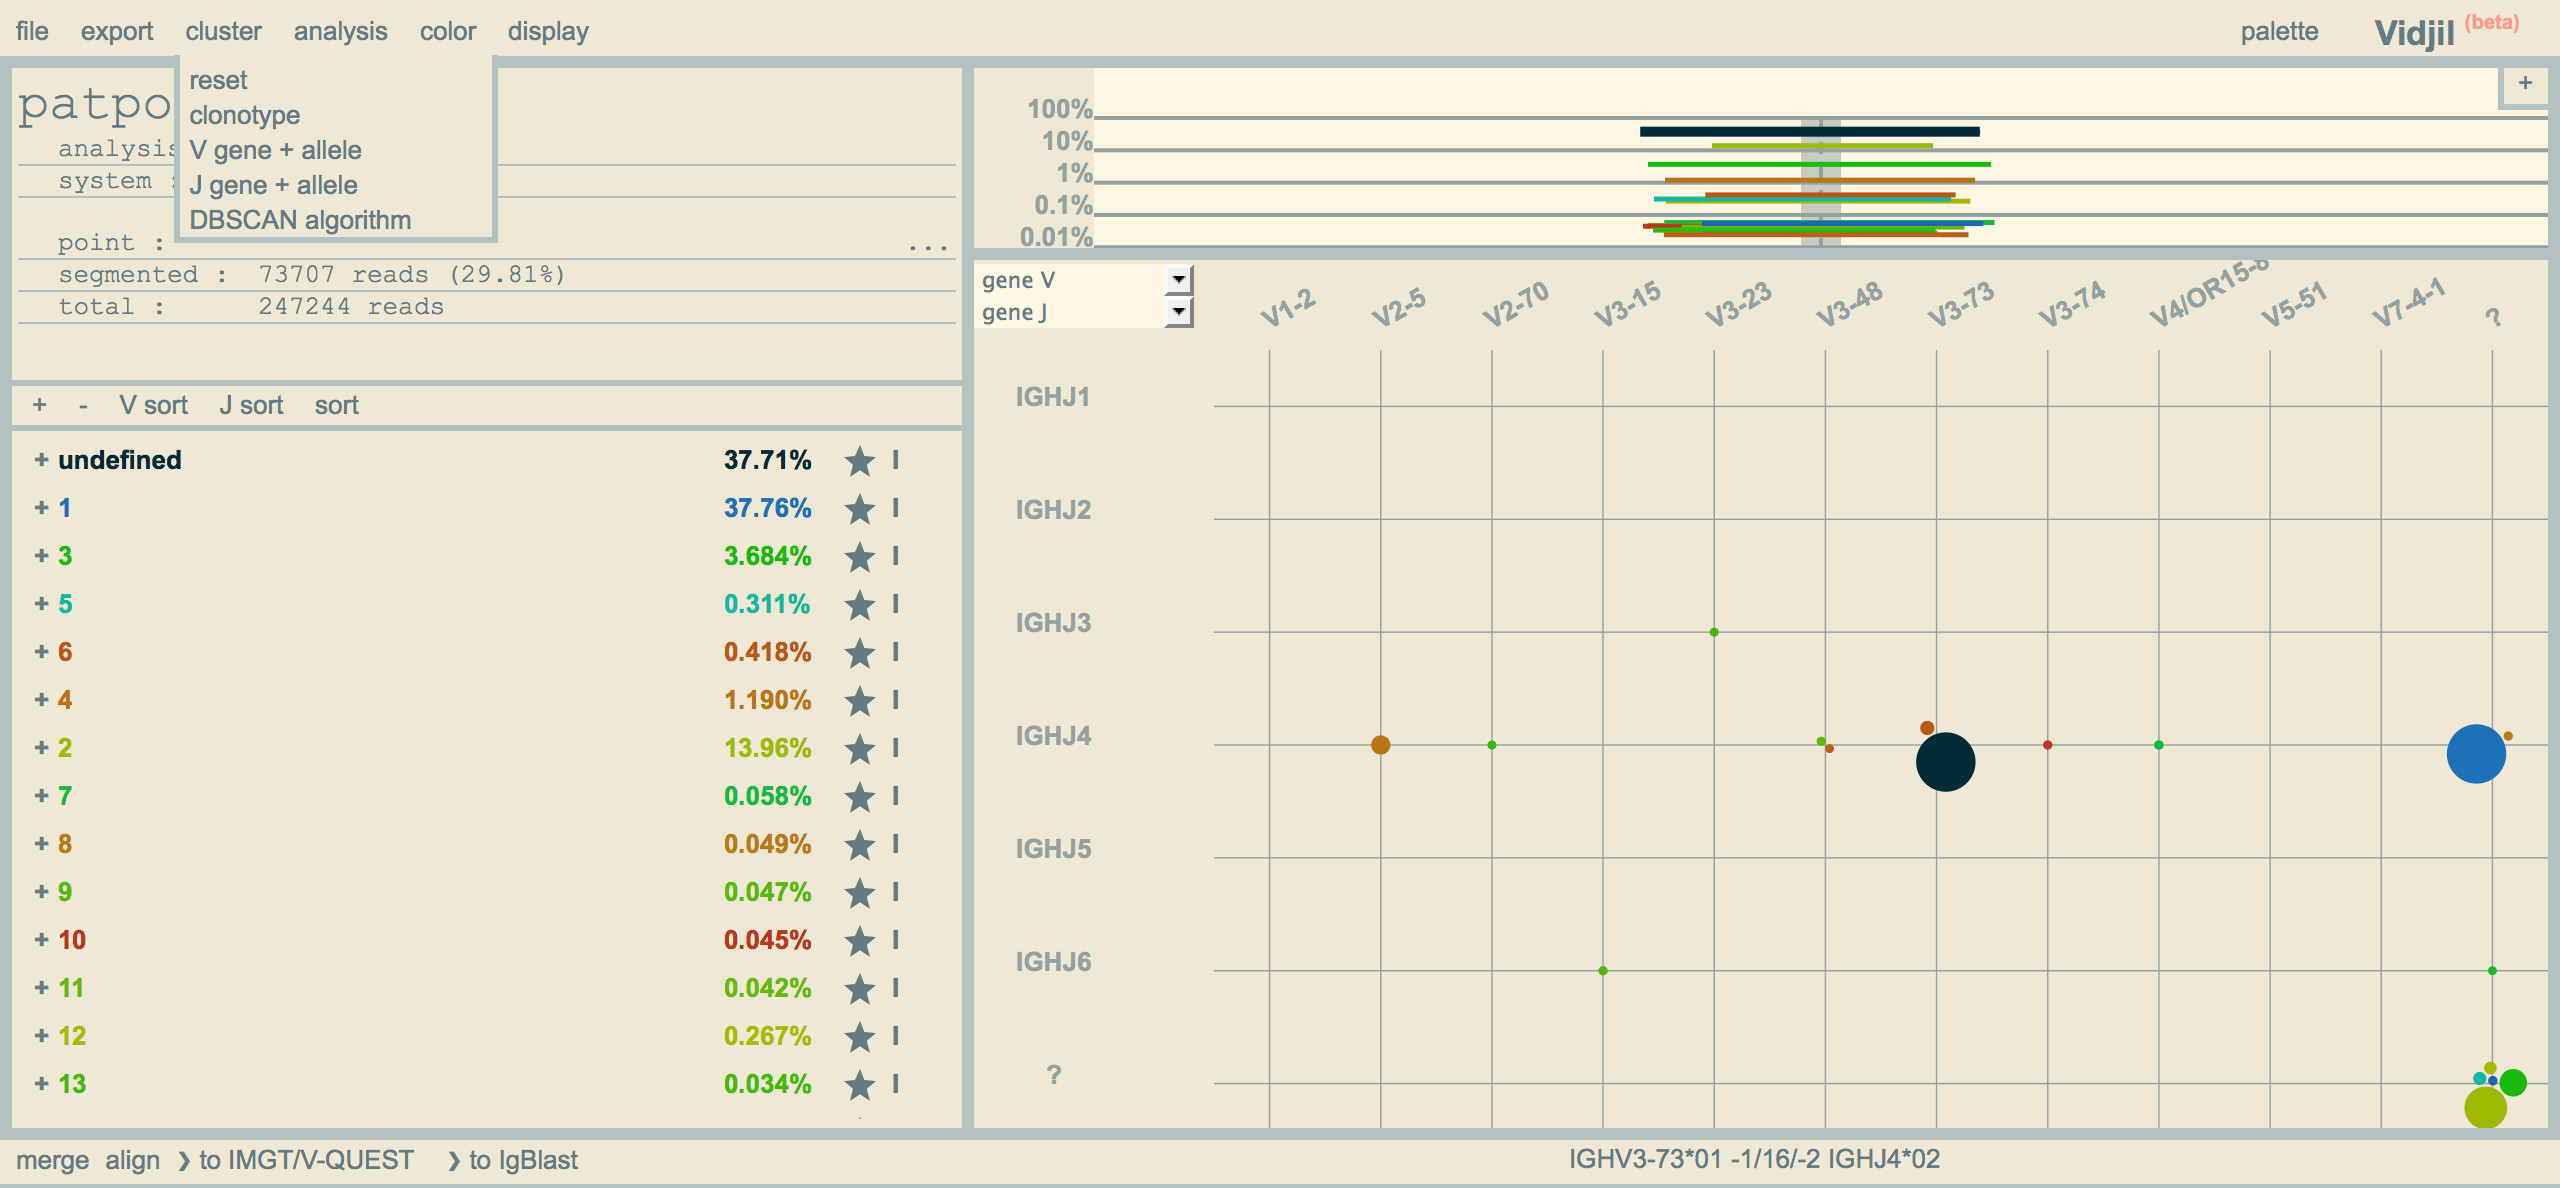
\includegraphics[scale=0.45]{img/DBSCAN-Cluster-Ex.jpg}
}
\end{center}
\caption{\textit{Afficheur} avec la clusterisation DBSCAN}
\end{figure}

\begin{figure}[h]
\begin{center}
\rotatebox{90}{
	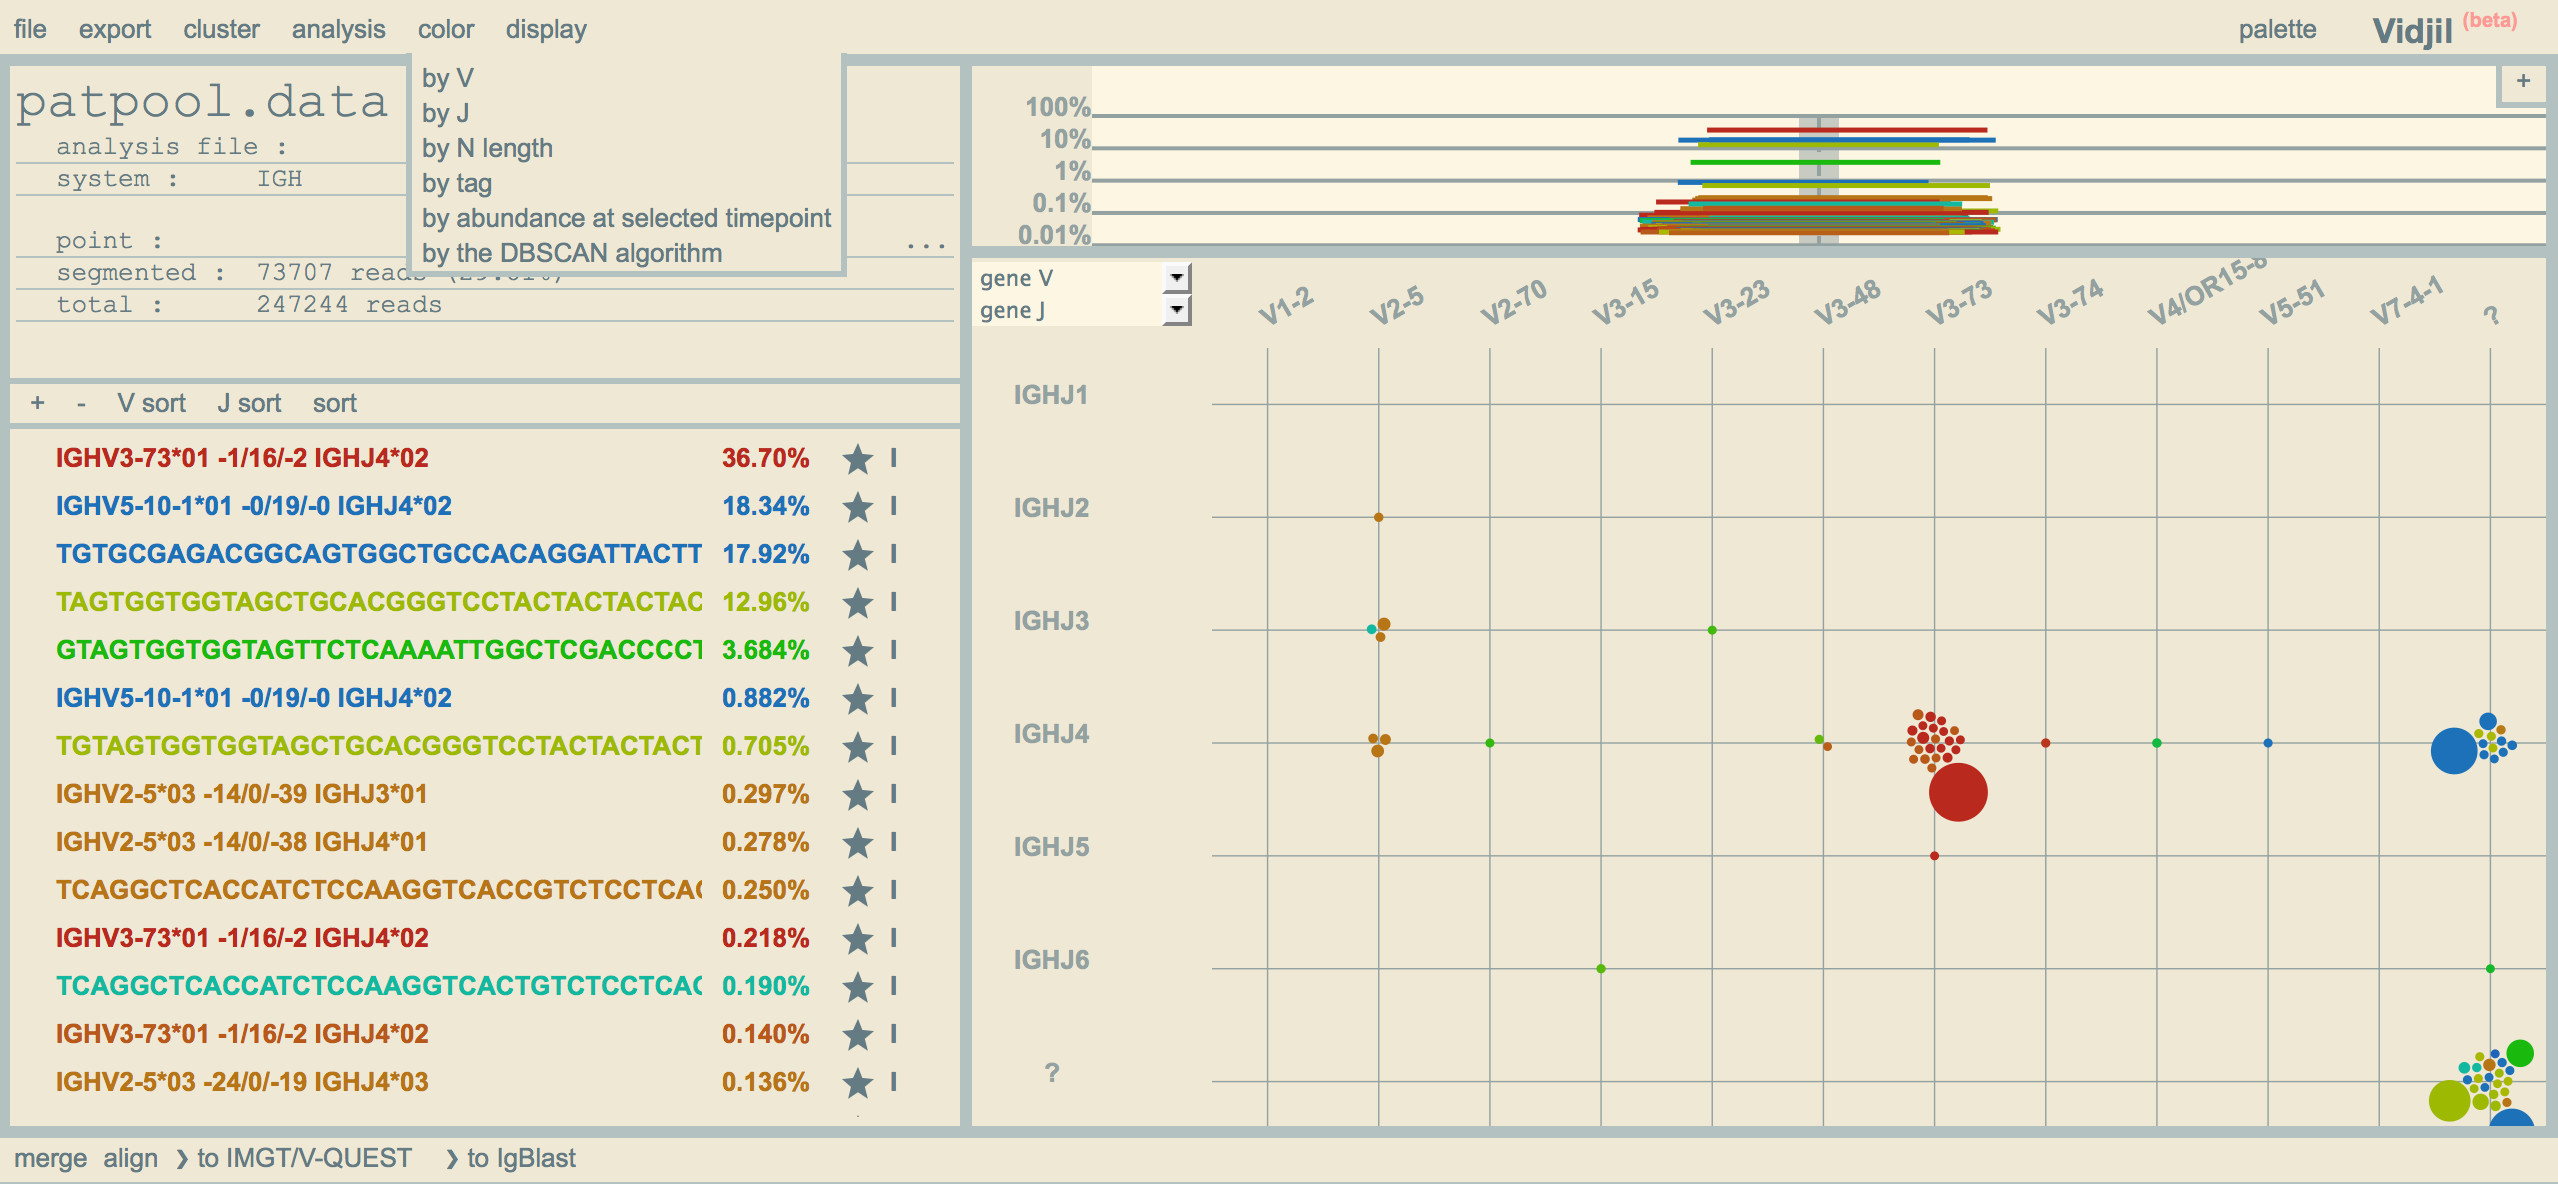
\includegraphics[scale=0.45]{img/DBSCAN-Color-Ex.jpg}
}
\end{center}
\caption{\textit{Afficheur} avec la colorisation DBSCAN}
\end{figure}

\begin{figure}[h]
\begin{center}
\rotatebox{90}{
	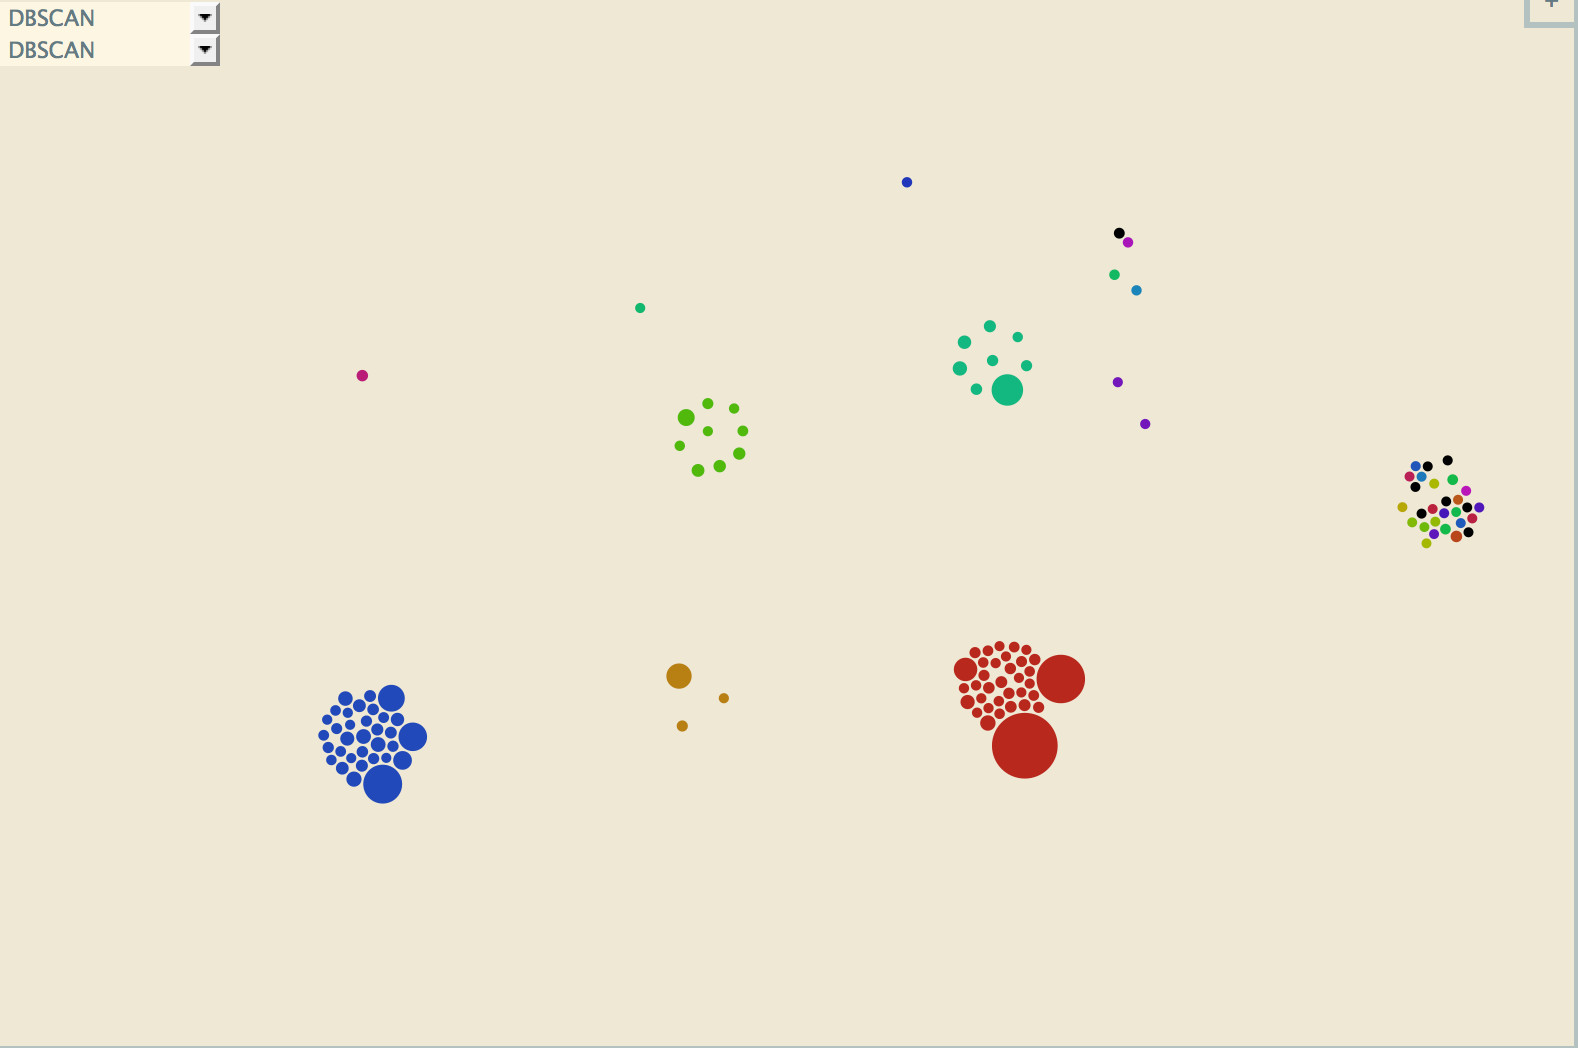
\includegraphics[scale=0.7]{img/DBSCAN-Ex.jpg}
}
\end{center}
\caption{\textit{Afficheur} avec la distribution DBSCAN}
\end{figure}

\chapter*{Recherche de la meilleure distance possible}

\addcontentsline{toc}{chapter}{Recherche de la meilleure distance possible}

\end{document}